\begin{center}
    \begin{large}
    Cp 8 - Recursividad\\
    Curso \academicyear\\
    \end{large}
    % \begin{figure}[h]
    % 	\centering
    % 	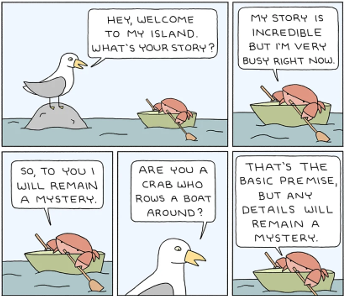
\includegraphics[width=0.5\linewidth]{cp5/classes.png}
    % \end{figure}
\end{center}

\section{Factorial}
El factorial de un número $n$ (denotado como $n!$) se define como el producto de todos los números enteros positivos desde 1 hasta $n$, o sea:

\[
n! = \prod_{k=1}^{n} k
\]

o lo que es lo mismo:

\[
n! =
\begin{cases} 
1 & \text{si } n = 0 \\
n \cdot (n-1)! & \text{si } n > 0
\end{cases}
\]

Implemente un programa que reciba un número entero no negativo \(n\) de la consola y calcule el factorial de ese número.

\subsection*{Ejemplos:}
\begin{itemize}
    \item Entrada: \texttt{0}\\
          Salida: \texttt{El factorial de 0 es 1.}
    \item Entrada: \texttt{1}\\
          Salida: \texttt{El factorial de 1 es 1.}
    \item Entrada: \texttt{5}\\
          Salida: \texttt{El factorial de 5 es 120.}
    \item Entrada: \texttt{7}\\
          Salida: \texttt{El factorial de 7 es 5040.}
\end{itemize}


\section{Cantidad de dígitos}
Implemente un método que reciba un número entero y halle su cantidad de dígitos (no usar la clase `string`).

% \[ CantidadDigitos(n) = \begin{cases}
% 1 & \text{si } n < 10 \\
% 1 + CantidadDigitos(\lfloor n / 10 \rfloor) & \text{de lo contrario}
% \end{cases} \]


\section{Suma de Dígitos}
Implementa un método que calcule recursivamente la suma de los dígitos de un úmero natural \( n \). Si \(n\) tiene \(d\) dígitos, representados por \(d_1, d_2, \ldots, d_d\), entonces la suma de los dígitos \(S(n)\) se define como:

$$
S(n) = \sum_{i=1}^{d} d_i
$$

Donde \(d_i\) representa el i-ésimo dígito de \(n\).


\section{Potencia}
Dado dos enteros $a$ y $b$, calcule el resultado de $a^b$.


\section{Máximo común divisor}
Implemente un método que halle el \textit{máximo común divisor} entre dos enteros utilizando el algoritmo de Euclides basado en el resto.

El \(mcd(a, b)\) es el mayor número \(d\) que divide a \(a\) y a \(b\) simultáneamente. Si \(a = b \cdot q + r\), donde:
\[
\begin{aligned}
q &\in \mathbb{Z}, \quad \text{(el cociente debe ser un número entero)} \\
0 &\leq r < b, \quad \text{(el residuo \(r\) es un número no negativo y estrictamente menor que \(b\))}.
\end{aligned}
\]
entonces:
\[
mcd(a, b) = mcd(b, r).
\]
Esto se debe a que cualquier divisor común de \(a\) y \(b\) también divide \(r\), y viceversa.


\section{Sucesión de Fibonacci}
Hallar el n-ésimo término de la sucesión de Fibonacci:

\[ F_0 = 1 \]
\[ F_1 = 1 \]
\[ F_n = F_{n-1} + F_{n-2} ~ para ~ n > 1 \]


\section{Secuencia de Collatz}
Escriba un programa que lea un número entero \( n \) de la consola e imprima la secuencia de Collatz para \( n \).

La secuencia de Collatz se define como:

\[ S_0 = n \]
\[ S_{n+1} = \left\{ \begin{array}{lcc}
             3 S_n + 1 ~ si ~ S_n ~ impar \\
             \\ \frac{S_n}{2} ~ si ~ S_n ~ par
             \end{array}
   \right. \]

Dicha secuencia termina cuando se alcanza el número \( 1 \).


\section{Superprimo}
Implemente un método que determine si un número es \texttt{super primo}. Un número es \texttt{super primo} si es primo y además al quitarle la última cifra sigue siendo \texttt{super primo}. Un número primo de una sola cifra se considera \texttt{super primo}. Ejemplo, 73 es superprimo.


\section{Representación binaria}
\begin{enumerate}[label=\alph*)]
    \item Implemente un método que convierta un número de binario a decimal. (El número binario está representado por un string compuesto de 0s y 1s).
    \item Implemente un método que reciba un número entero no negativo y devuelva un string con su representación binaria.
\end{enumerate}

\begin{enumerate}[label=\alph*)]
    \item Implemente un método que convierta un número de binario a decimal.\\
    Un número binario es una representación en base 2 de un número entero. El número binario está compuesto solo por los dígitos \(0\) y \(1\), donde cada posición en el número tiene un valor que es una potencia de 2, comenzando desde la derecha (posición 0).

    Para convertir un número binario a decimal, se puede utilizar la siguiente fórmula:
    \[
    n = \sum_{i=0}^{k} b_i \cdot 2^i
    \]
    donde \(b_i\) es el \(i\)-ésimo dígito del número binario, comenzando desde la derecha, y \(k\) es el índice de la posición más significativa (la izquierda).

    \subsection*{Ejemplos}
    \begin{itemize}
        \item Entrada: \( \text{1101} \) \\
        Salida: \( 13 \) \\
        Explicación:
        \[
        1101_2 = 1 \cdot 2^3 + 1 \cdot 2^2 + 0 \cdot 2^1 + 1 \cdot 2^0 = 8 + 4 + 0 + 1 = 13.
        \]
        El número binario \(1101_2\) equivale a \(13\) en decimal.

        \item Entrada: \( \text{10101} \) \\
        Salida: \( 21 \) \\
        Explicación:
        \[
        10101_2 = 1 \cdot 2^4 + 0 \cdot 2^3 + 1 \cdot 2^2 + 0 \cdot 2^1 + 1 \cdot 2^0 = 16 + 0 + 4 + 0 + 1 = 21.
        \]
        El número binario \(10101_2\) equivale a \(21\) en decimal.
    \end{itemize}

    \item Implemente un método que reciba un número entero no negativo y devuelva un string con su representación binaria.\\
    El número binario correspondiente se obtiene dividiendo el número entre 2 repetidamente, y registrando los restos de cada división. El número binario es el conjunto de los restos en orden inverso.

    \subsection*{Ejemplos}
    \begin{itemize}
        \item Entrada: \( 13 \) \\
        Salida: \( \text{1101} \) \\
        Explicación:
        \[
        \begin{aligned}
        13 \div 2 &= 6, \quad \text{resto } 1 \\
        6 \div 2 &= 3, \quad \text{resto } 0 \\
        3 \div 2 &= 1, \quad \text{resto } 1 \\
        1 \div 2 &= 0, \quad \text{resto } 1
        \end{aligned}
        \]
        Los restos en orden inverso son \(1101\), por lo tanto, la representación binaria de \(13\) es \(1101\).

        \item Entrada: \( 21 \) \\
        Salida: \( \text{10101} \) \\
        Explicación:
        \[
        \begin{aligned}
        21 \div 2 = 10,\quad \text{ resto } 1 \\
        10 \div 2 = 5,\quad\quad\quad \text{ resto } 0 \\
        5 \div 2 = 2,\quad\quad \text{ resto } 1 \\
        2 \div 2 = 1,\quad \text{ resto } 0 \\
        1 \div 2 = 0,\quad \text{ resto } 1
        \end{aligned}
        \]
        Los restos en orden inverso son \(10101\), por lo tanto, la representación binaria de \(21\) es \(10101\).
    \end{itemize}
\end{enumerate}


\section{Descomposición en factores primos}  
Dado un número \( n \). Hallar su descomposición en factores primos. Dicha descomposición consiste en el producto de potencias de factores primos tal que se obtenga el número.
  

\section{Echo invertido}
Implemente un método que permita al usuario escribir en la consola tantas líneas como quiera. Cuando el usuario de ''ENTER'' sin haber escrito algún texto, debe imprimir cada una de las líneas que escribió el usuario, pero en orden inverso. No debe usar array ni ninguna estructura de datos para almacenar todas las líneas de texto que ha ido escribiendo el usuario.

\section{Torres de Hanoi}
¿Recuerdas el problema de las Torres de Hanoi? Este consiste en mover una pila de discos de una torre a otra, respetando las siguientes reglas:
\begin{itemize}
    \item Solo se puede mover un disco a la vez.
    \item Un disco nunca puede colocarse sobre otro más pequeño.
    \item Solo se puede usar una torre auxiliar.
\end{itemize}

Escribe un método recursivo para resolver el problema de las Torres de Hanoi, mostrando los movimientos de los discos.

\textbf{Ejemplo:}\\
Si tienes 3 discos, la secuencia de movimientos sería:
\begin{itemize}
    \item Mover disco 1 de A a C
    \item Mover disco 2 de A a B
    \item Mover disco 1 de C a B
    \item Mover disco 3 de A a C
    \item Mover disco 1 de B a A
    \item Mover disco 2 de B a C
    \item Mover disco 1 de A a C
\end{itemize}

\section{Paréntesis balanceados}
Implemente un método que, dado un entero n, calcule la cantidad de cadenas (de paréntesis abiertos y cerrados) balanceadas de longitud $2 \cdot n$.

Una cadena de paréntesis está balanceada si:
\begin{itemize}
    \item Cualquier subcadena que comienza en el principio tiene un número de paréntesis abiertos mayor o igual que el número de paréntesis cerrados.
    \item La cadena tiene el mismo número de paréntesis abiertos que cerrados.
\end{itemize}

\texttt{((()))} es una cadena balanceada y \texttt{())(()} no lo es.

\subsection*{Ejemplos}

Para \( n = 3 \), hay 5 cadenas:
\begin{itemize}
    \item \( ((())) \)
    \item \( (()()) \)
    \item \( (())() \)
    \item \( ()(()) \)
    \item \( ()()() \)
\end{itemize}
